\documentclass{article}
\usepackage{graphicx} % Required for inserting images
\usepackage{amsmath} % for the cases environment

\title{Labwork3's report}
\author{Hai Nguyen Ngoc}
\date{May 3 2024}

\begin{document}
\maketitle

\section{Introduction}
Logistic regression is method for classification task. We calculate the predicted value by:

\begin{equation}
\sigma(z) = \frac{1}{1 + e^{-z}}
\end{equation}

With \(z = (w_1 \times x_{i}^{(1)} + w_2 \times x_{i}^{(2)} + w_0)\). Because we have 2 possible outputs, so that the error (or loss) functions can be calculated by:
\begin{equation}
L_i = 
\begin{cases} 
- \log(y_i) & \text{if } y_i = 1 \\
- \log(1 - y_i) & \text{if } y_i = 0 
\end{cases}
\end{equation}

And finally we have combination of above equation for 1 data point:

\begin{equation}
L_i = -(y_i \cdot \log(y_i) + (1 - y_i) \cdot \log(1 - y_i))
\end{equation}

For \(n\) data points, we have Loss function:

\begin{equation}
J = -\frac{1}{N} \sum_{i=1}^{N} \left( y_i \cdot \log(y'_i) + (1 - y_i) \cdot \log(1 - y'_i) \right)
\end{equation}

\section{Implementation}
\subsection{Functions}
\begin{itemize}
    \item First, we need to write predicted value as equation (1)
    \item Second, write function for loss function as equation (4)
    \item Functions for gradient descent as below equations: 

\begin{equation}
\frac{\partial L_i}{\partial w_0} =
\left( \frac{y_i}{y_i'} + \frac{-1 + y_i}{1 - y_i'} \right) \cdot \left[ -e^{- (w_1 x_i^{(1)} + w_2 x_i^{(2)} + w_0 )} / \left( 1 + e^{-(w_1 x_{i}^{(1)} + w_2 x_{i}^{(2)} + w_0 )}\right)^2 \right]
\end{equation}

\begin{equation}
\frac{\partial L_i}{\partial w_1} =
\left( \frac{y_i}{y_i'} + \frac{-1 + y_i}{1 - y_i'} \right) \cdot \left[ -e^{- (w_1 x_i^{(1)} + w_2 x_i^{(2)} + w_0 )} / \left( 1 + e^{-(w_1 x_{i}^{(1)} + w_2 x_{i}^{(2)} + w_0 )}\right)^2 \right] \cdot x_i^{(1)}
\end{equation}

\begin{equation}
\frac{\partial L_i}{\partial w_2} =
\left( \frac{y_i}{y_i'} + \frac{-1 + y_i}{1 - y_i'} \right) \cdot \left[ -e^{- (w_1 x_i^{(1)} + w_2 x_i^{(2)} + w_0 )} / \left( 1 + e^{-(w_1 x_{i}^{(1)} + w_2 x_{i}^{(2)} + w_0 )}\right)^2 \right] \cdot x_i^{(2)}
\end{equation}

    \item Write function to optimize parameters by Gradient Descent:
\begin{equation}
w_0 = w_0 - \alpha* \frac{\partial L_i}{\partial w_0}
\end{equation}
\begin{equation}
w_1 = w_1 - \alpha* \frac{\partial L_i}{\partial w_1}
\end{equation}
\begin{equation}
w_2 = w_2 - \alpha* \frac{\partial L_i}{\partial w_1}
\end{equation}
\end{itemize}

\subsection{Main}
Create initial value for \(w_0, w_1, W_2\):
\(w_0 = 1\),
\(w_1 = 2\),
\(w_2 = 0\),
Then loop until reach expected value or max number of iterations.

\section{Evaluation}
\begin{figure}
    \centering
    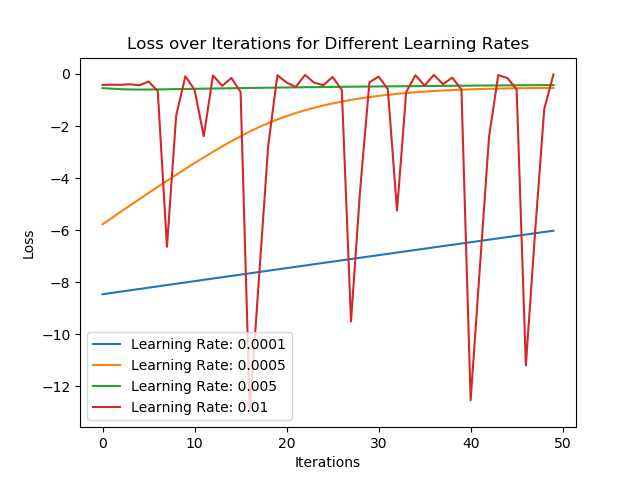
\includegraphics[width=0.75\linewidth]{01.png}
    \caption{Value of Loss function through iterations with different values of learning rate}
    \label{fig:enter-label}
\end{figure}

\section{Conclusion}
\begin{itemize}
\item Logistic regression work well in binary classification. 
\item Easy to implement and need to choose appropriate value of learning rate
\item Need to do carefully in partial derivative of \(w_0, w_1, w_2\)
\end{itemize}

\end{document}
